\chapter{Entscheidungsfindung} % (fold)
\label{cha:Entscheidungsfindung}

\section{Verwendete Methoden} % (fold)
\label{sec:Verwendete Methoden}

Verwendete Methoden
Um eine fundierte und stichhaltige Entscheidung treffen zu können und diese auch angemessen begründen zu können, haben wir uns für eine Nutzwertanalyse entschieden.

Eine Nutzwertanalyse ist eine Methode zur Entscheidungsfindung und wird häufig in komplexen Situationen verwendet, wenn beispielsweise viele verschiedene Aspekte und Meinungen betrachtet werden müssen. \footcite[Vgl.][S. 1 auch im Folgenden]{Kuhnapfel.2019} Sie beruht auf dem Prinzip der „Fragmentierung“, das bedeutet das Gesamtproblem wird in einzelne Teilprobleme aufgeteilt, die, wenn dies sinnvoll ist, noch einmal in ihre Teilprobleme aufgeteilt werden können. Dieses intuitive Modell wird häufig unterbewusst angewendet, wenn wir beispielsweise entscheiden wohin wir in den Urlaub möchten. Es können objektive Informationen, wie in diesem Beispiel Kosten oder Freizeitangebote, aber auch subjektive, wie Vorlieben für Essen oder Unterkunft betrachtet und miteinander abgewogen werden. \footcite[Vgl.][S. 43]{Dittmer.1995}

Durch das Erstellen einer Nutzwertanalyse wird dieser unterbewusste Prozess in den Vordergrund gebracht und der Fokus auf die Transparenz der Ergebnisse gelegt. Des Weiteren bewirkt die Fragmentierung eine Entemotionalisierung des Problems. Die Teilprobleme lenken von der emotionalen Bindung oder von einer spontanen Präferenz der Gesamtlösung ab und können leichter rational betrachtet und diskutiert werden. Dies ist vor allem der Fall, wenn der Anteil der Teillösung an der Gesamtlösung nicht klar ist. \footcite[Vgl.][S. 2]{Kuhnapfel.2019} Besonders der tendenziellen Präferenz sich für die Konstanz und gegen Veränderung zu entscheiden, wird hier entgegengewirkt.
Für eine zielführende Durchführung einer Nutzwertanalyse ist eine klar festgelegte Struktur notwendig, an der sich orientiert werden kann. Der erste und wichtigste Schritt ist die Ableitung des Zielsystems. \footcite[Vgl.][S. 44 f. auch im Folgenden]{Dittmer.1995} Ein Zielsystem setzt sich aus den bestimmten Kriterien zusammen und sollte eindeutige und objektive Beschreibungen der Wirkungen und Konsequenzen von Alternativen erlauben und alle relevanten Wertevorstellungen der Entscheidungsträger umfassen. Bei der Findung helfen Prozessfragen, wie beispielsweise „Welche Wirkungen werden beabsichtigt?“, „Worauf wirken die Alternativen?“, oder „Welche Wirkungen sollen vermieden werden?“.

Im Anschluss werden Ausschluss- und Auswahlkriterien definiert. Hier beginnt man mit Ausschlusskriterien, diese werden nicht in die Nutzwertanalyse mit einfließen, sondern schließen die Alternative kategorisch aus (auch K.O. Kriterien genannt). Auswahlkriterien können grundsätzlich in Leistungs-, Kosten-, und Terminkriterien eingeteilt werden, wobei in dieser Arbeit noch fachspezifische Kriterien betrachtet werden. \footnotemark
\footnotetext{Vgl. \cite{Wikipedia.2022} und \cite{FfEMunchen.2022}}
Eine Menge von 10-20 Kriterien wird als sinnvoll betrachtet, vor allem um zu verhindern, dass später besprochene Kriterien oberflächlicher behandelt und diskutiert werden als zu Beginn besprochene. \footcite[Vgl.][S. 8]{Kuhnapfel.2019}

Folgende Anforderungen werden an Kriterien in einer Nutzwertanalyse gestellt: \footnotemark
\footnotetext{Vgl. \cite{Kuhnapfel.2019} und \cite{Wikipedia.2022} auch im Folgenden}

\begin{description}
	\item \emph{Vollständigkeit:} Die Kriterien müssen das Problem vollständig umfassen, es darf also kein relevanter Aspekt für das Problem ausgelassen werden.
	\item \emph{Bewertbarkeit:} Kriterien sollten insofern bewertbar sein, als dass sie entweder qualitativ oder quantitativ erfassbar oder messbar sind, oder alle Teilnehmenden über das nötige Hintergrundwissen verfügen müssen, um eine informierte Bewertung abgeben zu können. Alternativ kann mit Enthaltungen gearbeitet werden, wenn beispielsweise ein sehr technischer und ein wirtschaftlicher Teil von zwei verschiedenen Abteilungen beurteilt wird.
	\item \emph{Relevanz:} Die Kriterien sollten für das in Frage stehende Problem relevant sein. Hier kann allerdings häufig keine eindeutige Aussage getroffen werden, da Teilnehmende hier eventuell andere Ansichten haben und oft keine objektive Antwort vorliegt.
	\item \emph{Reproduzierbarkeit:} Die verwendeten Kriterien sollten in ihrer Bewertung reproduzierbar sein. Das ist beispielsweise nicht der Fall, wenn die Verlässlichkeit einer Bank betrachtet wird und diese aktuell durch einen Sturm so verwüstet wurde, dass sie vorerst nicht handlungsfähig ist. Solange der Grund für die Unbeständigkeit nicht am Zielsystem selbst liegt ist das Kriterium unbrauchbar.
\end{description}

Im nächsten Schritt wird jedem Kriterium eine Gewichtung zu geordnet. Auch hier finden verschiedene Methoden Anwendung. Die einfachste aber auch ungenaueste Methode ist das „Ranking“, oder „Direct Ranking“. Hierbei wird jedem Kriterium ein Rang gegeben. Der Bereich der Aufstellung spielt hier keine große Rolle, ist im Beispiel (Abb. \ref{abb:DirectRanking}) aber mit 0-10 definiert.

\begin{figure}[htb]
	\centering
	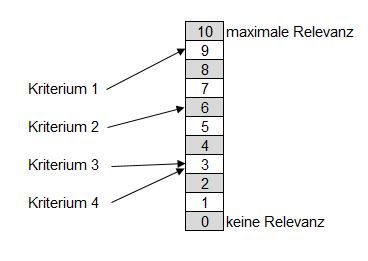
\includegraphics[width=5cm]{graphics/Direct_Ranking_Methode.JPG}
	\caption[Grafisches Beispiel Direct Ranking]{Grafisches Beispiel Direct Ranking. \footnotemark}
	\label{abb:DirectRanking}
\end{figure}
\footnotetext{Entnommen aus \cite{Wikipedia.2022}}

Die Kriterien 1-4 werden zwischen 0 (keine Relevanz) und 10 (maximale Relevanz) einsortiert. Diese Methode wird häufig verwendet, da sie so einfach ist und schnell erstellt werden kann, allerdings nimmt die Aussagekraft mit steigender Kriterienzahl stark ab. Zudem wird jedes Kriterium isoliert für sich betrachtet. Das bedeutet, es ist nicht möglich zu überprüfen inwiefern die Gewichtung passend ist. \footnotemark
\footnotetext{Vgl. \cite{PhilippsUniversitatMarburg.2013} und \cite{Wikipedia.2022}}

Des Weiteren kann durch ein sogenanntes Rating eine Gewichtung bestimmt werden. Bei diesem Verfahren kann man entweder eine Gesamtpunktzahl („Point Allocation“) auf die Kriterien aufteilen, beispielsweise 100 Punkte auf fünf Kriterien mit der Gewichtung 35, 30, 20, 10, 5. Die andere Möglichkeit ist die Verhältnisschätzung („Ratio Estimation“). Jedes Kriterium kann hier einer beliebigen Zahl aus dem Wertebereich zugeordnet werden. Das unwichtigste Kriterium beispielsweise der Punktzahl null, das wichtigste die zehn. \footcite[Vgl. ][]{PhilippsUniversitatMarburg.2013}

Für Nutzwertanalysen mit vielen Kriterien (ab ca. 20 definitiv) ist die Paarvergleichsmethode sehr sinnvoll.

\begin{table}[htb]
	\centering
	\begin{tabular}{|l||l|l|l|l|l|l|l||l|}
		\hline
		\textbf{Kriterium} & A & B & C & D & E  & F & G & $\sum$      \\
		\hline \hline
		A                  & ~ & 7 & 4 & 2 & 5  & 9 & 4 & \textbf{31} \\
		\hline
		B                  & 3 & ~ & 3 & 7 & 10 & 6 & 5 & \textbf{34} \\
		\hline
		C                  & 6 & 7 & ~ & 8 & 8  & 9 & 6 & \textbf{44} \\
		\hline
		D                  & 8 & 3 & 2 & ~ & 7  & 5 & 3 & \textbf{28} \\
		\hline
		E                  & 5 & 0 & 2 & 3 & ~  & 3 & 4 & \textbf{17} \\
		\hline
		F                  & 1 & 4 & 1 & 5 & 7  & ~ & 8 & \textbf{26} \\
		\hline
		G                  & 6 & 5 & 4 & 7 & 6  & 2 & ~ & \textbf{30} \\
		\hline
	\end{tabular}
	\caption[Kreuztabelle zur Gewichtung von Kriterien mit \glqq Ist-wichtiger-als \glqq -Stimmen]{Kreuztabelle zur Gewichtung von Kriterien mit \glqq Ist-wichtiger-als \grqq -Stimmen. \footnotemark}
	\label{tab:KreuztabelleKriterien}
\end{table}
\footnotetext{Entnommen aus \cite{Kuhnapfel.2019} S. 15}

Hier wird, wie in Tabelle \ref{tab:KreuztabelleKriterien} beispielhaft dargestellt, eine Kreuztabelle erstellt. Alle Teilnehmenden sollten einzeln bestimmen, welches Kriterium sie jeweils für wichtiger halten. Die Ergebnisse werden dann vom Moderator zusammengestellt und präsentiert. In diesem Fall haben zehn Teilnehmer abgestimmt. Logischerweise werden Kriterien nicht mit sich selbst verglichen, deshalb sind diese Felder ausgegraut. Die Ergebnisse sind hier in der letzten Spalte dargestellt und sind die Summe der „Ist-wichtiger-als“-Stimmen pro Kriterium. Im letzten Schritt wird wie in Tabelle \ref{tab:ErgebnisKreuztabelle} das Beispiel weitergeführt. Mit Hilfe eines Dreisatzes werden die Ergebnisse in ein Verhältnis gebracht und die Gewichtung berechnet. \footcite[Vgl. ][S. 13 ff.]{Kuhnapfel.2019}

\begin{table}
	\centering
	\begin{tabular}{l|l|l}
		~              & Stimmen & Gewicht(\%) \\
		\hline \hline
		Kriterium A    & 31      & 14,7        \\
		\hline
		Kriterium B    & 34      & 16,2        \\
		\hline
		Kriterium C    & 44      & 21,0        \\
		\hline
		Kriterium D    & 28      & 13,3        \\
		\hline
		Kriterium E    & 17      & 8,1         \\
		\hline
		Kriterium F    & 26      & 12,4        \\
		\hline
		Kriterium G    & 30      & 14,3        \\
		\hline
		\textbf(Summe) & 210     & 100         \\
		\hline
	\end{tabular}
	\caption[Ergebnis der Kriteriengewichtung auf Basis der Kreuztabelle]{Ergebnis der Kriteriengewichtung auf Basis der Kreuztabelle \footnotemark}
	\label{tab:ErgebnisKreuztabelle}
\end{table}
\footnotetext{Entnommen aus \cite{Kuhnapfel.2019} S. 16}

Bevor nun die Kriterien bewertet werden können, muss eine Skala bestimmt werden. Grundsätzlich hat die Skala keine Auswirkungen auf das Ergebnis der Nutzwertanalyse. Dennoch ist davon abzuraten sehr kleine oder sehr große Skalen zu definieren. Kleine Skalen bieten zu wenig Differenzierbarkeit, große hingegen können dafür sorgen, dass Teilnehmende, die zu Polarisierung neigen, mehr Einfluss auf das Ergebnis nehmen, als diejenigen, die sich tendenziell an der „goldenen Mitte“ orientieren. Die sicherlich einfachsten und verständlichsten Skalen sind die 0-10 Skala und die Schulnotenskala. Beide eignen sich hervorragend für eine Nutzwertanalyse. \footnotemark
\footnotetext{Vgl. \cite{Kuhnapfel.2019} S. 16 ff., \cite{Dittmer.1995} S. 49 f. und \cite{FfEMunchen.2022}}

Um eine Nutzwertanalyse verwendbar und aussagekräftig zu machen sollte sie reproduzierbar sein. Dies kann nur durch eine ausführliche und gewissenhaft geführte Dokumentation gewährleistet werden. Diese soll für Außenstehende ein nachvollziehbarer Nachweis sein. Zum einen soll eine Nutzwertanalyse mit anderen Teilnehmenden, an anderen Standorten oder zu einem anderen Zeitpunkt wiederholt werden können. \footnotemark
\footnotetext{Vgl. \cite{Kuhnapfel.2019} S. 4 f. und \cite{Wikipedia.2022}}

In der Dokumentation sollen harte und weiche Faktoren so erklärt werden, dass beide nachvollziehbar sind. Harte Faktoren können mit betriebswirtschaftlichen Kennzahlen belegt werden. Man spricht hier von ökonomischer Objektivierung durch Kennziffern. Weiche Faktoren hingegen beinhalten beispielsweise Erfahrungswerte, Images, Stimmungen und Handlungsweisen. Sie sind nicht oder nur mit Hilfsindikatoren als Kennzahlen darstellbar und ergeben sich aus der Diskussion. \footcite[Vgl. ][S. 1 f.]{Prof.Dr.JanLies.2018}

% section Verwendete Methoden (end)

\section{Durchführung} % (fold)
\label{sec:Durchführung}

Da im Haus schon mehrere VPN-Lösungen im Gebrauch sind, die auch für eine Harmonisierung in Frage kommen, war recht schnell klar, was die Auswahlmöglichkeiten für das Entscheidungsproblem sind. Für die Harmonisierung der VPN-Einzelplätze für interne Mitarbeiter der Komm.One kommen die Checkpoint-VPN Lösung und die NCP-VPN Lösung in Frage. Anyconnect-VPN, was auch in der Firma verwendet wird wurde bereits im Voraus aussortiert und wird im Folgenden nicht mehr betrachtet. Der enorme Aufwand eines kompletten Neuaufbaus und die damit verbundenen Kosten konnten den anderen beiden Alternativen von vornerein keine Konkurrenz machen.

Um alle benötigten Kriterien zu finden, haben wir die Methode des „Brainstorming“ verwendet. Daraus entstand folgende Liste: Fixe Kosten, Laufende Kosten, Anschaffungskosten Software, Anschaffungskosten Hardware, Softwarekosten einmalig, Softwarekosten laufend, Betriebskosten, Implementierungskosten, Migrationskosten, Kosten Kunde einmalig, Kosten Kunde laufend – Supportkosten, Skalierungskosten, Mitarbeiterkosten, Shared Service Kosten, Kostensumme innerhalb der nächsten 5 Jahre, Fortbildungskosten, Zeitaufwand Umstellung, Zeitaufwand Support, Einrichtung, Supportaufwände im Kalenderjahr, Supportaufwände einzeln, Administrationsaufwände, Rest-API (Funktion), Interkonnektivität (Funktion), Nutzung für Kunden, Self-Service Möglichkeiten, Sicherheit, Zuverlässigkeit, Handhabung, Anwenderfreundlichkeit und Verwaltungsfreundlichkeit.

Mit dieser Liste konnten wir dann weiterarbeiten. Sinn eines „Brainstormings“ ist es natürlich nicht sich viele Gedanken über die einzelnen Punkte zu machen, sondern möglichst alles, was den Beteiligten einfällt, fest zu halten. Viele dieser Punkte bedingen sich gegenseitig, oder meinen schlichtweg Dasselbe. Diese müssen natürlich entfernt werden. Einige der Punkte haben sich im Verlauf des Verfahrens als irrelevant, oder nicht umfangreich genug herausgestellt. Bei einigen wurde uns auch bewusst, dass sie genauer definiert werden müssen, um Missverständnisse zu vermeiden.

Ergebnis des Überarbeitungsprozesses ist die Tabelle \ref{tab:FinalKriterien}.

\begin{table}
	\centering
	\begin{tabular}{l|l|}
		                                       & \textbf{Kriterien}                  \\
		\hline \hline
		\multirow{10}{6em}{\textbf{Kosten}}    & Anschaffungskosten Software         \\
		~                                      & Anschaffungskosten Hardware         \\
		~                                      & Fortbildungskosten                  \\
		~                                      & Laufende Softwarekosten             \\
		~                                      & Laufende Hardwarekosten             \\
		~                                      & Mitarbeiterkosten einmalig          \\
		~                                      & Mitarbeiterkosten laufend           \\
		~                                      & Supportkosten                       \\
		~                                      & Skalierungskosten                   \\
		~                                      & Kosten für Fremdleistungen          \\
		\cline{2-2}
		\multirow{6}{6em}{\textbf{Aufwand}}    & Zeitaufwand Vorbereitung            \\
		~                                      & Zeitaufwand Implementierung         \\
		~                                      & Zeitaufwand Support                 \\
		~                                      & Anzahl Supportfälle im Kalenderjahr \\
		~                                      & Zeitaufwand pro Supportfall         \\
		~                                      & Administrationsaufwände             \\
		\cline{2-2}
		\multirow{2}{6em}{\textbf{Funktionen}} & Rest-API/Schnittstelle              \\
		~                                      & Interkonnektivität                  \\
		\cline{2-2}
		\multirow{7}{6em}{\textbf{Andere}}     & Self-Service                        \\
		~                                      & Sicherheit                          \\
		~                                      & Zuverlässigkeit                     \\
		~                                      & Anwenderfreundlichkeit              \\
		~                                      & Verwaltungsfreundlichkeit           \\
		~                                      & Fehlertoleranz Admin                \\
		~                                      & Fehlertoleranz Benutzer             \\
		\cline{2-2}
	\end{tabular}
	\caption[Finale Aufstellung aller verwendeten Kriterien für die Nutzwertanalyse]{Finale Aufstellung aller verwendeten Kriterien für die Nutzwertanalyse}
	\label{tab:Kriterien}
\end{table}

Die Punkte Anschaffungskosten Software und Hardware sind selbsterklärend, ebenso wie laufende Software- und Hardwarekosten. Bei den Fortbildungskosten geht es um Kosten für Schulungen für die Mitarbeiter, die bisher mit einer der anderen Lösungen gearbeitet haben. Mitarbeiterkosten einmalig bezieht sich auf die Kosten, die durch die Umstellung einmalig entstehen, während Mitarbeiter laufend die benötigten Mitarbeiter für den dauerhaften Betrieb der jeweiligen Lösung bewerten soll. Unter dem Kriterium Supportkosten wird bewertet, wie gut die jeweilige Alternative in Bezug auf die Menge an Supportanfrage an den Hersteller und die damit verbundenen Zusatzkosten ist. Auf den ersten Blick scheinen Kosten für Fremdleistungen hier das gleiche zu meinen, allerdings betrachten wir unter diesem Aspekt nicht die Kosten für Supportfälle und andere Unregelmäßigkeiten, sondern die Kosten, die regelmäßig für Arbeiten am System entstehen, aber nicht intern durchgeführt werden können. Skalierungskosten bezieht die Möglichkeit in Betracht das System in Zukunft erweitern zu können. Wie teuer wäre es beispielsweise das System um 500 Clients zu erweitern?

Zeitaufwände für Vorbereitung beschreibt den benötigten Zeitaufwand vor der Harmonisierung, um diese überhaupt möglich zu machen. Beim Zeitaufwand für Implementierung ist vor allem der Aspekt der Fehlerbehebung wichtig. Wie groß wird der Aufwand sein, um bei allen Mitarbeitern eine erneut funktionierende VPN-Verbindung aufbauen zu können? Zeitaufwand Support beschreibt die benötigte Zeit, die Mitarbeitende mit Supportfällen anderer Mitarbeitenden aufwenden müssen. Hierunter fallen auch Kleinigkeiten, wie Passwort vergessen oder ähnliches. Anzahl Supportfälle im Kalenderjahr und Zeitaufwand pro Supportfall sind aufgelistet der Vollständigkeit und Transparenz wegen, finden aber, wie später noch einmal genauer erläutert, keine eigene Gewichtung, sondern fließen unter dem Punkt Zeitaufwand Support in die Wertung mit ein. Drei Kriterien, die den gleichen Aspekt bewerten, verzerren das Ergebnis, wenn sie vollständig in das Ergebnis einfließen. Der Aspekt Support wäre deutlich wichtiger gewertet als gewünscht. Beispielsweise können zwei Alternativen hier eine ähnliche Bewertung was den Zeitaufwand für Support angeht bekommen, aber aus komplett verschiedenen Gründen. Bei Alternative A gibt es im Jahr nur zwei bis drei Supportfälle, diese sind aber immer sehr aufwendig und beanspruchen teilweise sogar mehrere Tage. Alternative B hat hingegen viele Supportfälle, die sich allerdings immer innerhalb einer halben Stunde beheben lassen. Da beide Alternativen in Summe auf ähnliche Zeitaufwände für Support kommen, ist die Bewertung zwar gleich, die Gründe hierfür sind allerdings so verschieden, dass wir das auch noch in Betracht ziehen wollen. Administrationsaufwände bezieht sich auf die Möglichkeiten Administrationsarbeiten, wie Updates oder sicherheitsrelevante Arbeiten durchzuführen.

Bei Rest-API/Schnittstelle geht es um eine Programmierschnittstelle, die das Verbinden mit Cloud-Diensten und Interaktionen ermöglicht. Bei dem Aspekt Interkonnektivität betrachten wir welche Geräte bzw. Betriebssysteme unterstützt werden. Speziell, ob Android- und Apple-Geräte unterstützt werden.

Self-Service bewertet die Möglichkeit, dass Mitarbeitende kleine Supportfälle, wie beispielsweise ein vergessenes Passwort und damit verbundenes gesperrtes Konto, selbst beheben können. Natürlich ist einer der wichtigsten Aspekte die Sicherheit. Anwenderfreundlichkeit bezieht sich zu großen Teilen auf persönliche Präferenzen, ebenso wie die Verwaltungsfreundlichkeit. Die Aspekte Fehlertoleranz Admin und Benutzer sollen bewerten, wie schlimm ein Fehler der jeweiligen Gruppe oder Person wäre und wie groß die Auswirkungen eines Fehlers potenziell sind.

Im nächsten Schritt wird die Gewichtung der Entscheidungskriterien betrachtet und bewertet. Hier bedienen wir uns keiner der bereits genannten Methoden direkt. Als Vorbild dient das Entscheidungsformular der Firma Komm.One, in der eine kleine und relativ oberflächliche Tabelle vorgegeben ist. Die Tabelle unterscheidet die Kriterien Kunden-/Anwenderperspektive, Finanzperspektive, Prozessperspektive, Personal-/Potenzialperspektive, Markenwirkung/Image, Recht/Compliance und Konsequenzen/Synergien/Effekte. Die Tabelle gibt Prioritäten von 0 (spielt keine Rolle), 1 (kaum Einfluss), 2 (beachtenswert) und 3 (starker Einfluss) vor. Pro Kriterium kann dann die beste Alternative gekennzeichnet werden und es wird ein Ergebnis berechnet. Eben diese Gewichtung von null bis drei haben wir uns zu Nutze gemacht, dabei handelt es sich um eine Verhältnisschätzung.

Das Ergebnis zeigt Tabelle \ref{tab:Gewichtungen}. Wir haben uns gegen eine Gewichtung der einzelnen Kriterienkategorien entschieden (daher alle auf eins gesetzt), da ansonsten die Ergebnisse noch stärker auseinandergehen und dies nicht mehr repräsentativ für den Vergleich der Lösungen wäre. Anschaffungskosten haben wir jeweils mit zwei bewertet, da Kosten, vor allem so große, immer wichtig sind, es sich aber um einmalige Kosten handelt und es unser Ziel war, die auf lange Sicht, beste Lösung zu finden. Fortbildungskosten werden in unserer Nutzwertanalyse zwar noch geführt, aber durch die Gewichtung von null fließt die Bewertung nicht in das Gesamtergebnis ein. Entfernen wollten wir es, ähnlich wie bei der Anzahl Supportfälle und Zeitaufwand pro Supportfall nicht, um eine möglichst hohe Transparenz zu erreichen. Die Nutzwertanalyse soll zeigen, dass diese Aspekte berücksichtigt wurden, jedoch in unserem Fall keinen Einfluss auf das Ergebnis haben sollen. Bei den laufenden Kosten haben wir uns auch jeweils für eine Gewichtung von zwei entschieden, obwohl es sich um immer wiederkehrende Kosten handelt, weil wir hier ein bisschen mit den Grenzen der Gewichtungsskala in Berührung kommen. Wir sind der Meinung, dass die laufenden Kosten wichtiger sind als die Anschaffungskosten, vor allem auf lange Sicht. Allerdings sind sie nicht so wichtig wie eindeutige dreier Gewichtungen wie laufende Mitarbeiterkosten oder die Sicherheit. Da in unserer Skala keine Wertung zwischen zwei und drei möglich ist haben wir uns dafür entschieden auch die laufenden Kosten mit zwei zu gewichten. In unseren Augen ist die Differenz zu einer dreier Gewichtung höher als zu einer zweier. Einmalige Mitarbeiterkosten sehen wir als nicht so wichtig an und haben deshalb eine eins vergeben. Die bereits erwähnten laufenden Mitarbeiterkosten, Supportkosten und Kosten für Fremdleistungen müssen eindeutig mit drei gewichtet werden. Grund dafür ist, dass es sich hierbei um die größten Kostenpunkte handelt. Der Aspekt der Skalierungskosten wird mit zwei gewichtet, weil auch hier die Relevanz auf lange Sicht auf jeden Fall gegeben ist, aber eine Gewichtung mit drei nicht gerechtfertigt ist.

\begin{table}
	\centering
	\begin{tabular}{l|l|l|}
		                                       & \textbf{Kriterien}                  & \textbf{Gewichtung} \\
		\hline \hline
		\multirow{10}{6em}{\textbf{Kosten}}    & Anschaffungskosten Software         & 2                   \\
		~                                      & Anschaffungskosten Hardware         & 2                   \\
		~                                      & Fortbildungskosten                  & 2                   \\
		~                                      & Laufende Softwarekosten             & 2                   \\
		~                                      & Laufende Hardwarekosten             & 2                   \\
		~                                      & Mitarbeiterkosten einmalig          & 2                   \\
		~                                      & Mitarbeiterkosten laufend           & 2                   \\
		~                                      & Supportkosten                       & 2                   \\
		~                                      & Skalierungskosten                   & 2                   \\
		~                                      & Kosten für Fremdleistungen          & 2                   \\
		\cline{2-3}
		\multirow{6}{6em}{\textbf{Aufwand}}    & Zeitaufwand Vorbereitung            & 2                   \\
		~                                      & Zeitaufwand Implementierung         & 2                   \\
		~                                      & Zeitaufwand Support                 & 3                   \\
		~                                      & Anzahl Supportfälle im Kalenderjahr & 0                   \\
		~                                      & Zeitaufwand pro Supportfall         & 0                   \\
		~                                      & Administrationsaufwände             & 2                   \\
		\cline{2-3}
		\multirow{2}{6em}{\textbf{Funktionen}} & Rest-API/Schnittstelle              & 1                   \\
		~                                      & Interkonnektivität                  & 2                   \\
		\cline{2-3}
		\multirow{7}{6em}{\textbf{Andere}}     & Self-Service                        & 2                   \\
		~                                      & Sicherheit                          & 3                   \\
		~                                      & Zuverlässigkeit                     & 3                   \\
		~                                      & Anwenderfreundlichkeit              & 3                   \\
		~                                      & Verwaltungsfreundlichkeit           & 3                   \\
		~                                      & Fehlertoleranz Admin                & 0                   \\
		~                                      & Fehlertoleranz Benutzer             & 3                   \\
		\cline{2-3}
	\end{tabular}
	\caption[Gewichtung der Kriterien mit der Skala 0-3]{Gewichtung der Kriterien mit der Skala 0-3}
	\label{tab:Gewichtungen}
\end{table}

Was den Zeitaufwand für die Vorbereitung und für die Implementierung angeht, haben wir uns auch hier für eine Gewichtung von zwei entschieden. Die Kriterien müssen natürlich in einem Verhältnis zum Nutzen der Umstellung stehen, sollen allerdings nicht entscheidend für das Endergebnis sein. Sicherlich einer der wichtigsten Punkte und ein großer Grund wieso die Harmonisierung vorangetrieben wird, sind die Supportaufwände für die jeweilige Alternative. Deshalb wird dieses Kriterium zweifelsohne mit drei gewichtet. Allerdings setzt sich hier das Kriterium aus den zwei nachfolgend aufgeführten Kriterien zusammen, die wir, wie bereits erwähnt, der Vollständigkeit und Transparenz wegen mit in der Nutzwertanalyse führen, sie aber nicht im Einzelnen in das Ergebnis einfließen lassen. Den Aspekt der Administrationsaufwände haben wir mit zwei gewichtet, mit einer ähnlichen Begründung, wie bei den laufenden Kosten. Es handelt sich definitiv um einen wichtigen Punkt, allerdings in unseren Augen nicht wichtig genug für eine Gewichtung von drei.
Die Funktion Rest-API/Schnittstelle haben wir mit eins bewertet, da sie einem einiges an Arbeit abnehmen und das Arbeiten vereinfachen kann, aber nicht notwendig ist. Die Interkonnektivität zwischen Geräten bzw. Betriebssystemen wird mit zwei gewichtet. Innerhalb der Firma wird größtenteils mit Windows gearbeitet, da aber einzelne Mac oder Linux Geräte vorhanden sind ist es sicherlich ein Aspekt der beachtet werden muss.

Self-Service Möglichkeiten orientieren sich zwar stark an dem Gedankengang, der bei der Rest-API/Schnittstelle Anwendung gefunden hat. Allerdings haben wir uns hier für eine Gewichtung von zwei entschieden, da dies abgesehen von den „Nice-To-Have“-Gründen enormen Einfluss auf Supportaufwände und -kosten haben kann. Sicherheit muss ohne Frage eine drei zugeordnet werden, ebenso wie der Zuverlässigkeit. Mit Zuverlässigkeit ist hier nicht nur die dauerhafte Möglichkeit einen VPN-Tunnel aufbauen zu können oder die Beständigkeit des Tunnels nach dem Aufbau gemeint, sondern auch die Redundanz bei Fehlern im System. Es darf beispielsweise nicht sein, dass der Ausfall eines Standortes für einen Zusammenbruch des ganzen Netzwerks führt und kein Mitarbeiter mehr arbeiten kann. Zusammen mit der Anwenderfreundlichkeit und der Verwaltungsfreundlichkeit können auch diese Aspekte alle Einfluss auf die Supportaufwände und –kosten haben und werden deshalb mit drei gewichtet. Fehlertoleranz des Admins ist ein weiterer Punkt, den wir der Vollständigkeit und Transparenz wegen aufgenommen haben, der aber nicht in das Ergebnis miteinfließt. Der Grund ist hier ganz klar, dass ein Admin mit jedem System, dass er betreut so umgehen kann, dass angemessen damit gearbeitet wird. Anders sieht das bei der Fehlertoleranz der Benutzer aus. Diesen Aspekt sehen wir auch aufgrund der Auswirkungen auf die Aspekte Supportaufwände und –kosten, aber auch direkt auf die Mitarbeiterkosten laufend als sehr wichtig und haben ihn deshalb mit drei gewichtet.

% section Durchführung (end)

\section{Ergebnisse} % (fold)
\label{sec:Ergebnisse}

% TODO: Verweise einfügen
Folgende Bewertungen haben wir vergeben (Tab. 5 und Tab. 6).

\begin{table}
	\centering
	\begin{tabular}{l|l|l|l|r|}
		\textbf{Checkpoint}                    & \textbf{Kriterien}                  & \textbf{Gewichtung} & \textbf{Bewertung} & \textbf{Ergebnis} \\
		\hline \hline
		\multirow{10}{6em}{\textbf{Kosten}}    & Anschaffungskosten Software         & 2                   & 10                 & 20                \\
		~                                      & Anschaffungskosten Hardware         & 2                   & 10                 & 20                \\
		~                                      & Fortbildungskosten                  & 2                   & 2                  & 0                 \\
		~                                      & Laufende Softwarekosten             & 2                   & 9                  & 18                \\
		~                                      & Laufende Hardwarekosten             & 2                   & 8                  & 16                \\
		~                                      & Mitarbeiterkosten einmalig          & 2                   & 5                  & 5                 \\
		~                                      & Mitarbeiterkosten laufend           & 2                   & 8                  & 24                \\
		~                                      & Supportkosten                       & 2                   & 7                  & 21                \\
		~                                      & Skalierungskosten                   & 2                   & 2                  & 4                 \\
		~                                      & Kosten für Fremdleistungen          & 2                   & 10                 & 30                \\
		\cline{2-5}
		\multirow{6}{6em}{\textbf{Aufwand}}    & Zeitaufwand Vorbereitung            & 2                   & 3                  & 6                 \\
		~                                      & Zeitaufwand Implementierung         & 2                   & 5                  & 10                \\
		~                                      & Zeitaufwand Support                 & 3                   & 7                  & 21                \\
		~                                      & Anzahl Supportfälle im Kalenderjahr & 0                   & 10                 & 0                 \\
		~                                      & Zeitaufwand pro Supportfall         & 0                   & 4                  & 0                 \\
		~                                      & Administrationsaufwände             & 2                   & 6                  & 12                \\
		\cline{2-5}
		\multirow{2}{6em}{\textbf{Funktionen}} & Rest-API/Schnittstelle              & 1                   & 6                  & 6                 \\
		~                                      & Interkonnektivität                  & 2                   & 4                  & 8                 \\
		\cline{2-5}
		\multirow{7}{6em}{\textbf{Andere}}     & Self-Service                        & 2                   & 4                  & 8                 \\
		~                                      & Sicherheit                          & 3                   & 10                 & 30                \\
		~                                      & Zuverlässigkeit                     & 3                   & 10                 & 30                \\
		~                                      & Anwenderfreundlichkeit              & 3                   & 5                  & 15                \\
		~                                      & Verwaltungsfreundlichkeit           & 3                   & 10                 & 30                \\
		~                                      & Fehlertoleranz Admin                & 0                   & 3                  & 0                 \\
		~                                      & Fehlertoleranz Benutzer             & 3                   & 9                  & 27                \\
		\cline{2-5}
	\end{tabular}
	\caption[Ergebnis der Nutzwertanalyse für Checkpoint-VPN]{Ergebnis der Nutzwertanalyse für Checkpoint-VPN}
	\label{tab:ErgebnisCheckpoint}
\end{table}

\begin{table}
	\centering
	\begin{tabular}{l|l|l|l|r|}
		\textbf{NCP}                           & \textbf{Kriterien}                  & \textbf{Gewichtung} & \textbf{Bewertung} & \textbf{Ergebnis} \\
		\hline \hline
		\multirow{10}{6em}{\textbf{Kosten}}    & Anschaffungskosten Software         & 2                   & 10                 & 20                \\
		~                                      & Anschaffungskosten Hardware         & 2                   & 10                 & 20                \\
		~                                      & Fortbildungskosten                  & 2                   & 2                  & 0                 \\
		~                                      & Laufende Softwarekosten             & 2                   & 4                  & 8                 \\
		~                                      & Laufende Hardwarekosten             & 2                   & 5                  & 10                \\
		~                                      & Mitarbeiterkosten einmalig          & 2                   & 5                  & 5                 \\
		~                                      & Mitarbeiterkosten laufend           & 2                   & 4                  & 12                \\
		~                                      & Supportkosten                       & 2                   & 4                  & 12                \\
		~                                      & Skalierungskosten                   & 2                   & 6                  & 12                \\
		~                                      & Kosten für Fremdleistungen          & 2                   & 6                  & 18                \\
		\cline{2-5}
		\multirow{6}{6em}{\textbf{Aufwand}}    & Zeitaufwand Vorbereitung            & 2                   & 3                  & 6                 \\
		~                                      & Zeitaufwand Implementierung         & 2                   & 2                  & 4                 \\
		~                                      & Zeitaufwand Support                 & 3                   & 3                  & 9                 \\
		~                                      & Anzahl Supportfälle im Kalenderjahr & 0                   & 1                  & 0                 \\
		~                                      & Zeitaufwand pro Supportfall         & 0                   & 5                  & 0                 \\
		~                                      & Administrationsaufwände             & 2                   & 6                  & 12                \\
		\cline{2-5}
		\multirow{2}{6em}{\textbf{Funktionen}} & Rest-API/Schnittstelle              & 1                   & 5                  & 5                 \\
		~                                      & Interkonnektivität                  & 2                   & 6                  & 12                \\
		\cline{2-5}
		\multirow{7}{6em}{\textbf{Andere}}     & Self-Service                        & 2                   & 4                  & 8                 \\
		~                                      & Sicherheit                          & 3                   & 10                 & 30                \\
		~                                      & Zuverlässigkeit                     & 3                   & 6                  & 18                \\
		~                                      & Anwenderfreundlichkeit              & 3                   & 6                  & 18                \\
		~                                      & Verwaltungsfreundlichkeit           & 3                   & 8                  & 24                \\
		~                                      & Fehlertoleranz Admin                & 0                   & 2                  & 0                 \\
		~                                      & Fehlertoleranz Benutzer             & 3                   & 6                  & 18                \\
		\cline{2-5}
	\end{tabular}
	\caption[Ergebnis der Nutzwertanalyse für NCP-VPN]{Ergebnis der Nutzwertanalyse für NCP-VPN}
	\label{tab:ErgebnisNCP}
\end{table}

Die Anschaffungskosten für sowohl Software, als auch Hardware, haben wir mit zehn bewertet. Aus dem Grund, dass keine Kosten dafür anfallen, weder für Checkpoint, noch für NCP. Die benötigte Hardware ist bereits in unseren Rechenzentren vorhanden und muss nur gebucht werden und keine der Alternativen fordert einmalige Kosten für den Aufbau des Systems. Die nicht in das Ergebnis einfließenden Fortbildungskosten haben wir mit jeweils zwei bewertet. In beiden Fällen müssen Mitarbeiter an Fortbildungen teilnehmen. Die laufenden Softwarekosten berufen sich auf zwei bereits eingeholte Angebote der Firmen. CP verlangt 13,28 € pro Client pro Jahr, was sich in unserem Fall, bei 1800 benötigten Clients auf 23.904,00 € pro Jahr beläuft. Zusätzlich dazu kommt eine Wartungspauschale von 1.020,00 €. Die gesamten laufenden Softwarekosten belaufen sich also auf 24.924,00 € pro Jahr. Dem entgegen steht das deutlich kompliziertere Modell von NCP. Nach dem wie oben bereits erklärten „Pay-Per-Use“-Modell von NCP belaufen sich nach unseren Berechnungen die laufenden Softwarekosten auf 59.250,88 € pro Jahr. Dieses Verhältnis von ungefähr 0,4 wollten wir in unserer Bewertung wiederspiegeln und haben deshalb neun und vier Punkte an jeweils Checkpoint und NCP vergeben. Die Bewertung der laufenden Hardwarekosten beruht auf einem internen Angebot unseres Rechenzentrums. Hierbei ist geplant für Checkpoint zwei virtuelle Maschinen mit jeweils 8vCPUs und 32 GB RAM einzusetzen. Wobei beide virtuellen Maschinen redundant zueinander sind, sie können also jeweils die gesamte Clientzahl übernehmen. Die Kosten hierfür belaufen sich auf 3.588,00 € pro virtuelle Maschine pro Jahr. Also insgesamt 7.176,00 € pro Jahr. Dagegen steht der für NCP benötigte Aufbau mit zwei Management-VMs und 6 Gateway-Servern, wobei immer jeweils zwei redundant arbeiten und bis zu 250 aktive Verbindungen ermöglichen. Die Kosten für einen Managementserver belaufen sich auf 2.364,00€ pro Jahr, während für die Gateways jeweils 1.272,00 € pro Jahr anfallen. Die laufenden Gesamtkosten für Hardware belaufen sich hier also auf 12360 € pro Jahr. Das entstehende Verhältnis von etwa 0,6 spiegelt sich auch hier in der Bewertung von acht für Checkpoint und fünf für NCP wieder.

Mitarbeiterkosten einmalig haben wir bei beiden Alternativen mit fünf bewertet, da in beiden Fällen Einweisungsarbeiten, jeweils für Token und Zertifikat, anfallen, ebenso wie die Kosten für die Implementierung selbst. Diese sind aber auf beiden Seiten ähnlich. Bei den laufenden Mitarbeiterkosten sieht das anders aus. Hier haben wir uns für eine Bewertung von acht für Checkpoint und nur vier für NCP entschieden. Gründe hierfür waren vor allem die im NCP-Client verwendeten Zertifikate. Diese laufen ein Jahr, werden aber bereits nach zehn Monaten erneuert, um den Mitarbeitern die Möglichkeit zu geben einen Monat Spielraum zur Abholung zu haben. Dies ist jedes Mal ein enormer Aufwand, der bei Checkpoint nicht existiert. Supportkosten haben wir mit sieben für Checkpoint und vier für NCP bewertet, was an den unterschiedlichen Preisen und an den unterschiedlichen Mengen an benötigten Supportstunden liegt. Checkpoint verlangt 160,00 € netto pro Stunde, während NCP bei 250,00 € netto pro Stunde liegt. Zudem kommt, dass bei Checkpoint seit April 2021 keine einzige Stunde in Anspruch genommen wurde. Dagegen wird intern bei NCP mit etwa 30.000 € pro Jahr gerechnet. Was Skalierungskosten anbelangt hat hier NCP besser abgeschnitten. Das System kann um jeweils zwei virtuelle Maschinen erweitert werden, die 250 aktive Verbindungen mehr zulassen würde. Bei Checkpoint müsste man die Kapazitäten verdoppeln. Deshalb haben wir Checkpoint mit zwei und NCP mit sechs bewertet. Da wir in der eigenen Firma viele Mitarbeiter haben, die über ein gutes Know-how von Checkpoint verfügen, fallen hier praktisch keine Kosten an. Anders ist das bei NCP, hier ist nur ein Experte im Unternehmen verfügbar. Aus diesem Grund haben wir die Kosten für Fremdleistungen mit zehn für Checkpoint und sechs für NCP bewertet.

Beim Zeitaufwand für die Vorbereitung lässt sich kein wesentlicher Unterschied feststellen. Beide Lösungen haben drei Punkte erhalten, was zu großen Teilen daran liegt, dass die Abteilungen mit ihrer täglichen Arbeit schon im Stress sind und der dadurch entstehende Mehraufwand nicht so einfach kompensiert werden kann. Im Zeitaufwand für die Implementierung punktet Checkpoint mit fünf Punkten ein bisschen besser als NCP mit zwei. Grund hierfür ist die Trennung von Mitarbeitern und Kunden im NCP System. Diesen Mehraufwand gibt es bei Checkpoint nicht. Der Zeitaufwand für Support liegt mit sieben bei Checkpoint und drei bei NCP auch relativ stark auf der Seite von Checkpoint. Das liegt vor allem an der Anzahl Supportfälle im Kalenderjahr. Hier liegt Checkpoint mit zehn zu eins vorn. Diese Differenz kann NCP auch nicht mit dem Zeitaufwand pro Supportfall ausgleichen, da sie hier nur mit einem Punkt besser abschneidet und fünf Punkte erhält. Hier zeigt sich nochmal, wieso es uns wichtig war diese beiden Aspekte anzuführen, obwohl sie nicht auf das Ergebnis einwirken. Im Aspekt der Administrationsaufwände lässt sich keine wesentliche Unterscheidung finden. Die Firewall hinter dem System ist dieselbe und die unterschiedlichen Management Konsolen lassen sich nicht als besser oder schlechter bewerten. Deshalb bekommen beide Alternativen hier sechs Punkte.

Die Funktion Rest-API/Schnittstelle ist bei Checkpoint zwar gegeben, wird aber aktuell nicht verwendet, da die Freischaltung über AD-Gruppen und somit über Benutzer und nicht über IPs erfolgt. Bei NCP wird die neue Version sogar über eine Rest-API mit Python-Schnittstelle verfügen, da diese aktuell allerdings noch nicht verfügbar ist, ist sie nicht vollständig in die Wertung eingeflossen. Checkpoint erhält hier sechs Punkte, NCP fünf. Der Checkpoint-Client funktioniert auf Mac- und Windows-Geräten, was die relevanten und wichtigen Teile des Unternehmens abdeckt. Da NCP allerdings zusätzlich noch Linux unterstützt erhält NCP hier sechs Punkte und Checkpoint nur vier.

Das Kriterium Self-Service wird jeweils mit vier bewertet, da beide Lösungen sehr ähnliche Leistungen bieten. Im Thema Sicherheit sind beide Alternativen sehr gut. Beide bieten Funktionen an, die über das hinausgehen, was wir als Firma brauchen und benutzen. Deshalb bekommen beide hier zehn Punkte. Was das Thema Zuverlässigkeit angeht liegt Checkpoint mit zehn Punkten deutlich vor NCP mit sechs Punkten. Checkpoint hat schlichtweg deutlich weniger Probleme als NCP. Anwenderfreundlichkeit haben wir mit fünf Punkten für Checkpoint und 6 Punkten für NCP bewertet. Beide Systeme sind leicht zu verwenden, allerdings hat NCP hier aufgrund der Zertifikate einen kleinen Vorteil. Der Anwender hat mit den Zertifikaten selbst nichts zu tun, während er beim Token wissen muss, wie dieser funktioniert und wie er ihn benutzt. In der Verwaltungsfreundlichkeit liegt Checkpoint allerdings wieder vorne. Der direkte Zusammenhang mit der Firewall funktioniert hier sehr gut und ist sehr übersichtlich. Laut Erfahrungsberichten gibt es nichts Besseres. Deshalb bekommt Checkpoint hier zehn Punkte. NCP funktioniert hier zwar auch problemlos, kann aber mit Checkpoint nicht mithalten und bekommt acht Punkte. Die Fehlertoleranz des Admins haben wir mit drei für Checkpoint und zwei für NCP bewertet. Für beide Alternativen sind Revisionen auf Seite der Firewall vorhanden, aber Checkpoint hat bei Veränderungen zwei benötigte Bestätigungen, während NCP nur eine verwendet. Außerdem dokumentiert Checkpoint übersichtlicher was verändert wurde, wann etwas verändert wurde und von wem es verändert wurde. Bei der Fehlertoleranz der Benutzer ist Checkpoint erneut relativ deutlich mit neun zu sechs voraus. Das liegt vor allem daran, dass Checkpoint IP-Wechsel ermöglicht, ohne eine Trennung der Verbindung. Das ist bei NCP nicht möglich. Außerdem hält Checkpoint die Verbindung sehr lange aufrecht, wenn eine schlechte Internetverbindung besteht. NCP steigt hier deutlich früher aus.

Das Gesamtergebnis zeigt einen deutlichen Vorteil von Checkpoint gegenüber NCP mit 459 zu 343 Punkten.

% section Ergebnisse (end)

\section{Diskussion} % (fold)
\label{sec:Diskussion}

Checkpoint hat mit 459 Punkten und einer Differenz von 116 Punkten ziemlich genau ein Drittel mehr Punkte erreicht als NCP. In der Kategorie Funktionen ist die Differenz am geringsten, hier liegt NCP sogar 3 Punkte vorne, sie ist allerdings die Kategorie mit am wenigsten vergebenen Punkten und den wenigsten Kriterien. Die größte Differenz zeigt sich bei den Kosten. Hier liegt Checkpoint mit 77 Punkten vorne. Prozentual betrachtet ist das allerdings nur der zweitgrößte Unterschied. In der Kategorie Aufwand hat Checkpoint mit 49 zu 31 Punkten 58% mehr Punkte als NCP, im Gegensatz zu 43% mehr Punkten in der Kategorie Kosten. Die Kategorie Andere ist mit den Punktzahlen 140 zu 116 und ca. 21% mehr Punkten für Checkpoint in beiden Bereichen im Mittelfeld.

Diesen Zahlen verstärken noch einmal das Bild, das sich im Gesamtergebnis zeigt. Checkpoint gewinnt mit großem Vorsprung und ist in nahezu allen Kategorien überlegen. Natürlich muss man dazu sagen, dass viele Aspekte, wie Zeitaufwand Support oder Verwaltungsfreundlichkeit auf Erfahrungswerten einiger weniger Mitarbeiter beruht. Es handelt sich hier um weiche Faktoren. Einige der Bewertungen sind durch eigene Erfahrungen und Präferenzen geprägt, was sich allerdings nicht vermeiden lässt. Nicht alle Mitarbeiter, die im VPN Bereich arbeiten, kennen sich mit allen Systemen gleich gut aus, geschweige denn alle anderen Mitarbeiter der Firma. Zudem kommt, dass einige, der von uns ausgewählten und auch sicherlich relevanten Kriterien, nicht objektiv zu bewerten sind. Die Bewertung für jegliche benötigten Zeitaufwände sind reine Schätzungen, die sich aus Erfahrungswerten zusammensetzen. Häufig liegen aber keine Zahlen oder andere Werte vor, die diese Bewertungen direkt stützen oder widerlegen können. 

Erfreulich für uns ist zu sehen, dass die Kosten, als harte Faktoren, einen so großen Unterschied machen. Das macht es auch einfacher den geplanten Schritt vor der Geschäftsführung zu vertreten. Die Wirtschaftlichkeit ist generell eines der wichtigsten, wenn nicht das wichtigste Entscheidungskriterium bei derartigen Entscheidungen.

% section Diskussion (end)

% chapter (end)
